\documentclass{patmorin}

\usepackage{pat}
\usepackage[utf8]{inputenc}
\usepackage[noend]{algorithmic}
\usepackage{subcaption}

\newcommand\numberthis{\addtocounter{equation}{1}\tag{\theequation}}

% taken from http://goo.gl/JVNEL2
\newtheorem{innercustomthm}{Theorem}
\newenvironment{customthm}[1]
  {\renewcommand\theinnercustomthm{#1}\innercustomthm}
  {\endinnercustomthm}

%\newcommand{\keywords}[1]{\vspace{2em}\noindent\textbf{Keywords:} #1}
%\newcommand{\from}{\colon}

\title{\MakeUppercase{Encoding Arguments}}
\author{Pat Morin, Tommy Reddad, and Wolfgang Mulzer}
\date{}

\begin{document}
\begin{titlepage}
\maketitle


\begin{abstract}
\setlength{\baselineskip}{15.84pt}
  This expository article surveys ``encoding arguments.'' In their
  most most basic form an encoding argument proves an upper bound on
  the probability of an event using the fact a uniformly random choice
  from a set of size $N$ can not be encoded with fewer than $\log N$
  bits on average.

  We survey many applications of this basic argument, give a
  generalization of this argument for the case of non-uniform
  distributions, and give a rigorous justification for the use of
  non-integer codeword lengths in encoding arguments.  These latter
  two results allow encoding arguments to be applied more widely and to
  produce tighter results.
\end{abstract}

\keywords{Encoding arguments, entropy, Kolmogorov complexity, 
          incompressibility, random graphs, expanders, \ldots}

\end{titlepage}
\pagenumbering{roman}
\tableofcontents
\newpage
\pagenumbering{arabic}

\section{Introduction}
\setlength{\baselineskip}{15.84pt}
There is no doubt that probability theory plays a fundamental role
in computer science: Some of the fastest and simplest fundamental
algorithms and data structures are randomized; average-case analysis of
algorithms relies entirely on tools from probability theory; and many
difficult combinatorial questions have strikingly simple solutions using
probabilistic arguments.

Unfortunately, many of these beautiful results are inaccessible
to most computer scientists because of a view that ``the math
is too hard.''  For instance, the 2013 edition of ACM/IEEE
Curriculum Guidelines for Undergraduate Degree Progams in Computer
Science does not require a full course in probability theory
\cite[Page~50]{computing-curricula:computer}. Indeed, the report
recommends a total of 6 Tier-1 hours and 2 Tier-2 hours spent on
discrete probability, as part of the discrete structures curriculum
\cite[Page~77]{computing-curricula:computer}.

In this expository paper, we survey applications of ``encoding arguments''
that tranforms the problem of upper-bounding the probability of a specific
event, $\mathcal{E}$, into the problem of devising a code for the set
of elementary events in 
$\mathcal{E}$.  Encoding arguments have several advantages over
traditional probabilistic analysis:

\begin{enumerate}
  \item Encoding arguments are almost ``probability-free.''  Except for
  applying a simple \emph{Uniform Encoding Lemma}, there is no probability
  involved.  In particular, there is no chance to make common mistakes
  such as multiplying probabilities of non-independent events or
  (equivalently) multiplying expectations.

  The proof of the Uniform Encoding Lemma itself is trivial and the only
  probability it uses is that the fact, if a finite set $X$ contains $r$
  special elements and we pick an element uniformly at random from $X$,
  then the probability of picking a special element is $r/|X|$.

  \item Encoding arguments usually yield strong results;
  $\Pr\{\mathcal{E}\}$ typically decreases at least exponentially in
  the parameter of interest. Traditionally, these strong concentration
  results require (at least) careful calculations on probabilities of
  independent events and/or the application of concentration inequalities.
  The subject of concentration inequalities is advanced enough to be
  the topic of entire textbooks \cite{boucheron.lugosi.ea:concentration,dubhashi.panconesi:concentration}.
  
  \item Encoding arguments are natural for computer scientists. They
  turn a probabilistic analysis problem into the problem of designing an
  efficient code---an algorithmic problem. Consider the following 
  two problems:
    \begin{enumerate}

    \item Prove an upper-bound of $1/n^{\log n}$ on the probability that
       a random graph on $n$ vertices contains a clique of size $k=\lceil
       4\log n\rceil$.

    \item Design a encoding for graphs on $n$ vertices so that a graph,
       $G$, that contains a clique of size $k=\lceil 4\log n\rceil$
       is encoded using at most $\binom{n}{2}-\log^2 n$ bits. (Note:
       Your encoding and decoding algorithms don't have to be efficient,
       just correct.)
    \end{enumerate}
  Many computer science undergraduates would not know where to start
  on the first problem.  Even a good student who realizes that
  they can use Boole's Inequality will still be stuck
  wrestling with the formula $\binom{n}{4\log n}2^{-\binom{k}{2}}$.  
\end{enumerate}

Our motivation for this work is that encoding arguments are an easily
accessible, yet versatile tool for answering many questions.  Most of
these arguments can be applied after learning almost no probability
theory beyond the Encoding Lemma mentioned above.

The remainder of this article is organized as follows: In \secref{uel},
we present necessary background, including the \emph{Uniform
Encoding Lemma}, which is the basis of most of our encoding arguments.
\Secref{applications-i} presents  applications of the Uniform Encoding
Lemma to a variety of problems.  \Secref{nuel} presents a more
general Non-Uniform Encoding Lemma that can handle a larger variety of
applications, some of which are presented in \secref{applications-ii}.
\Secref{weights} presents an alternative view of encoding arguments in
terms of weight functions; this alternative view justifies the use of
non-integer codeword lengths.  \Secref{summary} summarizes and concludes
with some directions for future research.



\section{Background}
\seclabel{uel}

This section presents the necessary background on prefix-free codes and binomial coefficients.

\subsection{Prefix-free Codes and the Uniform Encoding Lemma}

A \emph{code}, $C\from X\to \{0,1\}^*$ is a one-to-one function from a set
$X$ to the set of binary strings.  The elements of the range of $C$ are
called $C$'s \emph{codewords}.  In most cases, there are some elements of
the set $X$ that are not of interest to us.  In these cases, we consider
partial codes. A \emph{partial code} $C\from X\nrightarrow \{0,1\}^*$ is
a one-to-one partial function.  When discussing partial codes we will use
the convention that $|C(x)|=\infty$ if $x$ is not in the domain of $C$.

A (partial) code, $C$, is \emph{prefix-free} if, for every pair $x\neq y$
in the domain of $C$ the binary string $C(x)$ is not a prefix of $C(y)$.
It can be helpful to think of prefix-free codes as (rooted ordered)
binary trees whose leaves are labelled with the elements of $X$.
The codeword for a particular $x\in X$ is obtained by tracing the
root-to-leaf path leading to $x$ and outputting a 0 (respectively, 1)
each time this path goes from a parent to its left (respectively, right)
child. (See \figref{bintree}.)

\begin{figure}
  \centering{\includegraphics{bintree}}
  \caption{A prefix-free code for the set
    $X=\{\mathtt{a},\mathtt{b},\mathtt{c},\mathtt{d},\mathtt{e},\mathtt{f}\}$
    and the corresponding leaf-labelled binary tree. (Which can also be viewed as a prefix-free partial code for the set $\{\mathtt{a},\mathtt{b},\mathtt{c},\ldots,\mathtt{z}\}$.)}
  \figlabel{bintree}
\end{figure}

If $C$ is prefix-free, then the number of $C$'s codewords that have length
\emph{at most} $k$ is not more than $2^k$. To see this why this is so,
observe that $C$ can be modified into a code $\hat C$, in which every
codeword of length $\ell <k$ is extended---by appending $k-\ell$ zeros---so that
it has length exactly $k$. The prefix-freeness of $C$ ensures that $\hat
C$ is also a prefix-free code. The number of $\hat C$'s codewords of
length $k$ is equal to the the number of $C$'s codewords of length at
most $k$; since codewords are just binary strings, there are not more
than $2^k$ of these.

Observe that every finite set $X$ has a prefix-free code in which every
codeword has length $\lceil\log |X|\rceil$. We simply enumerate the
elements of $X$ in some order $x_0,x_1,\ldots,x_{|X|-1}$ and assign to
each $x_i$ the binary representation of $i$ (padded with leading zeros),
which has length $\lceil\log |X|\rceil$, since $i\in\{0,\ldots,|X|-1\}$.
We will use this type of \emph{fixed-length code} implicitly in many arguments.


As we will see, the following lemma, which is folklore, is surprisingly
versatile:
\begin{lem}[Uniform Encoding Lemma]\lemlabel{uel}
  Let $C\from X\nrightarrow \{0,1\}^*$ be a prefix-free partial code. If
  an element $x\in X$ is chosen uniformly at random, then $\Pr\{|C(x)|\le
  \log|X|-s\}\le 2^{-s}$.
\end{lem}

\begin{proof}
  Let $k=\log|X|-s$ and recall that $C$ has at most $2^{k}$ codewords
  of length at most $k$.  Since $C$ is one-to-one each such codeword has
  at most one preimage in $X$.  Since $x$ is chosen uniformly at random
  from $X$, the probability that it is the preimage of one of these
  short codewords is at most
  \[
     \frac{2^k}{|X|} = \frac{2^{\log|X|-s}}{|X|} = 2^{-s} \enspace . \qedhere 
  \]
\end{proof}

\subsection{Runs in Binary Strings}

As a warm-up exercise to illustrate the use of the Uniform Encoding
Lemma we will show that a random $n$-bit string is unlikely to contain
a run of significantly more than $\log n$ one bits.  (See \figref{runs-i}.)

\begin{figure}
  \centering{\includegraphics{runs-i}}
  \caption{Illustration of \thmref{runs-i} and its proof.}
  \figlabel{runs-i}
\end{figure}

\begin{thm}\thmlabel{runs-i}
  Let $x=(x_1,\ldots,x_n)\in\{0,1\}^n$ be chosen uniformly at random
  and let $t \ge \lceil\log n\rceil + s$. Then, the probability that
  there exists an $i\in\{1,\ldots,n-t+1\}$ such that
  $x_i=x_{i+1}=\cdots=x_{i+t-1}=1$ is at most $2^{-s}$.
\end{thm}

\begin{proof}
  We will prove this theorem by constructing a partial prefix-free
  code for strings having a run of $t$ or more 1's.  For such a string
  string $x=(x_1,\ldots,x_n)$ let $i$ be the minimum index such that
  $x_i=x_{i+1}=\cdots=x_{i+t-1}=1$. The codeword, $C(x)$, for $x$ is
  the binary string that consists of the
  ($\lceil\log (n - t)\rceil$-bit binary encoding of the) index $i$
  followed by the $n-t$ bits
  $x_1,\ldots,x_{i-1},x_{i+t},\ldots,x_n$. (see \figref{runs-i}.)

  Observe that $C(x)$ has length 
  \[
  \lceil\log (n - t)\rceil + n - t \le \lceil\log n\rceil + n - t \le
  n-s \enspace .
  \]
  It is easy to check that, for any such $x$, we can reconstruct
  $(x_1,\ldots,x_n)$ from $C(x)$, so $C$ is indeed a partial code
  whose domain is the set of binary strings of length $n$ having a run
  of $t$ or more 1's.  It is also easy to see that $C$ is prefix free,
  since all codewords are unique and have the same length.

  Now, $x$ was chosen uniformly at random from a set of size $2^{n}$.
  Therefore, by the Uniform Encoding Lemma, the probability that there
  exists any index $i\in\{1,\ldots,n-t-1\}$ such that
  $x_i=x_{i+1}=\cdots=x_{i+t-1}=1$ is at most
  \[
      \Pr\{|C(x)|\le n-s\} \le 2^{-s} \enspace . \qedhere 
  \]
\end{proof}

Simple as it is, the proof of \thmref{runs-i} contains the main ideas
used in most encoding arguments:

\begin{enumerate}
\item The arguments usually show that a particular \emph{bad event} is
  unlikely. In \thmref{runs-i} the bad event is the occurrence of a
  substring of $t$ consecutive 1's.

\item The code is partial prefix-free code whose domain contains the
  set of bad events. In this case, the code $C$ is only capable of
  encoding strings containing a run of $t$ consecutive 1's.

\item The code usually begins with a concise description of the bad
  event, and is then followed by a straightforward encoding of the
  information that is not implied by the bad event. In
  \thmref{runs-i}, the bad event is completely described by the index
  $i$ at which the run of $t$ 1 bits begins, and this implies that the
  bits $x_i,\ldots,x_{i+t-1}$ are all equal to 1, so these bits do not
  need to be specified in the second part of the codeword.
\end{enumerate}

\subsection{A Note on Ceilings}

Note that \thmref{runs-i} also has an easy proof using the union
bound: If we let $\mathcal{E}_i$ denote the event
$x_i=x_{i+1}=\cdots x_{i+t}=1$, then
\begin{align*}
\Pr \bigcup_{i=0}^{n-t-1} \mathcal{E}_i  
   & \le \sum_{i=0}^{n-t-1} \Pr\mathcal{E}_i & \text{(using the union bound)}\\
   & = \sum_{i=0}^{n-t-1} 2^{-t} & \text{(using the independence of the $x_i$'s)}\\
   & \le n2^{-t} & \text{(the sum has $n-t\le n$ identical terms)}\\
   & = n2^{-\lceil\log n\rceil-s} & \text{(from the definition of $t$)}\\
   & \le 2^{-s} \enspace .
\end{align*}
This traditional proof also works with the sometimes smaller value
$t=\log n+s$ (note the lack of a ceiling over the logarithmic term),
in which case the final inequality becomes an equality.

In the encoding proof of \thmref{runs-i}, the ceiling in the
expression for $t$ is an artifact of encoding of the integer $i$ which
is taken from a set of $n$. When sketching an encoding argument, we
think of this as requiring $\log n$ bits but when it comes time to
carefully write down a proof we include a ceiling over this term since
bits are a discrete quantity.

In \secref{weights}, however, we will see that the informal intuition
we use in blackboard proofs is actually valid; we can think of
encoding $i$ using $\log n$ bits even if $\log n$ is not an integer.
In general we can imagine encoding a choice from among $r$ options
using $\log r$ bits for any $r\in\N$.  From this point onwards, we
omit ceilings this way in all our theorems and proofs. This makes
calculations simpler and provides tighter results.  For now, it allows
us to state the following cleaner version of \thmref{runs-i}:

\begin{customthm}{\ref{thm:runs-i}b}\thmlabel{runs-ii}
  Let $x=(x_1,\ldots,x_n)\in\{0,1\}^n$ be chosen uniformly at random
  and let $t \ge \log n + s$. Then, the probability that there exists
  an $i\in\{1,\ldots,n-t+1\}$ such that
  $x_i=x_{i+1}=\cdots=x_{i+t-1}=1$ is at most $2^{-s}$.
\end{customthm}

\subsection{Encoding Sparse Bit Strings}

At this point we should also point out an extremely useful trick that
we can use for encoding sparse bit strings. For any $\alpha\in(0,1)$,
there exists a code $C_\alpha\from \{0,1\}^n\rightarrow \{0,1\}^*$
such that, for any bit string $x\in\{0,1\}^n$ having $n_1(x)$ 1's and
$n_0(x)$ 0's,
\begin{equation}
  |C_\alpha(x)| = \lceil n_1(x)\log(1/\alpha) + n_0(x)\log(1/(1-\alpha)) \rceil \enspace .
  \eqlabel{sparse-bitstring-i}
\end{equation}
This code is the so-called Shannon-Fano code for Bernoulli$(\alpha)$
bitstrings of length $n$
\cite{fano:transmission,shannon:mathematical}.

Again, as we will see in \secref{weights}, we can omit the ceiling in
the expression for $|C_\alpha(x)|$.  This is true for any value of
$n$. In particular, for $n=1$, it gives us a ``code'' for encoding a
single bit where the cost of encoding a 1 is $\log(1/\alpha)$ and the
cost of encoding a 0 is $\log(1/(1-\alpha))$.  Indeed, the ``code''
for bitstrings of length $n>1$ is just what we get when we apply this
1-bit code to each bit of the bitstring.

If we wish to encode bitstrings of length $n$ and we know in advance
that the strings have exactly $k$ 1 bits, then we can optimize this
process by taking $\alpha=k/n$, in which case we obtain a fixed length
code of length
\begin{equation}
    k\log (n/k) + (n-k)\log(n/(n-k))  \eqlabel{sparse-bitstring-ii} \enspace .
\end{equation}
\Eqref{sparse-bitstring-ii} brings us to our next topic: binary entropy.

\subsection{Binary Entropy}

The \emph{binary entropy function} $H\from (0,1)\to(0,1]$ is defined by
\[
    H(\alpha) = \alpha\log(1/\alpha) + (1-\alpha)\log(1/(1-\alpha)) 
\]
and will be quite useful.  The binary entropy function and two upper
bounds on it that we derive below are illustrated in \figref{entropy}.

\begin{figure}
  \centering{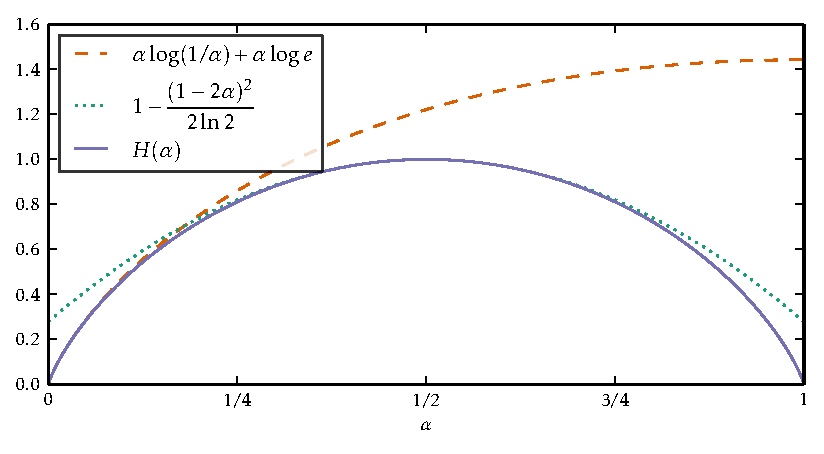
\includegraphics{entropy}}
  \caption{Binary entropy, $H$, and two useful approximations.}
  \figlabel{entropy}
\end{figure}

Notice that we have already encountered a quantity that can be expressed
in terms of the binary entropy.  From \eqref{sparse-bitstring-ii},
a bitstring of length $n$ that has exactly $k$ 1 bits can be encoded
with a fixed length code of length $nH(k/n)$.

The binary entropy function can be difficult to work with, so it is
helpful to have some manageable approximations.  One of these is derived
as follows:
\begin{align}
  H(\alpha) & = \alpha\log(1/\alpha) + (1-\alpha)\log(1/(1-\alpha)) \notag \\
       & = \alpha\log(1/\alpha) + (1-\alpha)\log(1+(\alpha/(1-\alpha)) \notag \\
       & \le \alpha\log(1/\alpha) + \alpha\log e \eqlabel{entropy-i} 
\end{align}
since $1+x\le e^x$ for all $x\in\mathbb{R}$. \Eqref{entropy-i} is a
useful approximation when $\alpha$ is close to zero, so that $H(\alpha)$ is also
close to zero.

For $\alpha$ close to $1/2$ (so that $H(\alpha)$ is close to 1), we
obtain a good approximation from the Taylor series expansion at $1/2$. In
particular, for $\alpha=(1-\epsilon)/2$,
\begin{align}
   H(\alpha) & = 1-\frac{1}{2\ln 2}\sum_{i=1}^{\infty}\frac{(1-2\alpha)^{2i}}{i(2i-1)} 
            \notag \\ 
        & = 1-\frac{1}{2\ln 2}\sum_{i=1}^{\infty}\frac{\epsilon^{2i}}{i(2i-1)} 
             \notag \\ 
        & < 1-\frac{\epsilon^2}{2\ln 2} \enspace .\eqlabel{entropy-ii}
\end{align}

\subsection{Basic Chernoff Bounds}

Since we now have the pieces we need, we give an encoding argument
for a well-known and extremely useful result typically attributed to
Chernoff \cite{X}.

\begin{thm}\label{chernoff-basic}
  Let $x=(x_1,\ldots,x_n)\in\{0,1\}^n$ be chosen uniformly at
  random.Then
  \[  \Pr\{n_1(x) \le n(1-\epsilon)/2\} < e^{-\epsilon^2n/2} \]
\end{thm}

\begin{proof}
Encode the bitstring $x$ using a Shannon-Fano code, $C_\alpha$, with
$\alpha=(1-\epsilon)/2$.  Then the length of the codeword for $x$ is
\[
     |C_\alpha(x)| = n_1(x)\log(1/\alpha) + n_0(x)\log (1/(1-\alpha))  \enspace .
\]
Since $\alpha < 1/2$, $\log(1/\alpha) > \log(1/(1-\alpha))$, so
$|C_\alpha(x)|$ is maximal when $n_1(x)$ is maximal.  Under the conditions
of the theorem, this happens when $n_1(x)=\alpha n$.  Therefore,
\begin{align*}
  |C_\alpha(x)| & \le \alpha n\log(1/\alpha) + (1-\alpha)n\log(1/(1-\alpha))\\
                & = n H(\alpha) \\
                & \le n\left(1-\frac{\epsilon^2}{2\ln 2}\right) \enspace ,
\end{align*}
where the second inequality is an application of \eqref{entropy-ii}.
Now, $x$ was chosen uniformly at random from a set of size $2^n$.
Therefore, this encoding saves:
\[  
    s = n-\left(n\left(1-\frac{\epsilon^2}{2\ln 2}\right)\right)
      = \frac{\epsilon^2n}{2\ln 2} 
\]
bits.  By the Uniform Encoding Lemma, the probability that this happens
is at most
\[
     2^{-s} = e^{-\epsilon^2n/2} \enspace . \qedhere
\]
\end{proof}
In \secref{chernoff}, after developing a Non-Uniform Encoding Lemma,
we will extend this argument to binary strings where each bit is set
independently to 1 or 0 with probabilities $p$ and $1-p$, respectively.

\subsection{Factorials and Binomial Coefficients}
\seclabel{stirling}

Before moving on to some more advanced encoding arguments, it will
be helpful to remind the reader of a few inequalities that can be
derived from Stirling's Approximation of $n!$.  Recall that Stirling's
Approximation states that
\begin{equation}
  n! = \left(\frac{n}{e}\right)^n\sqrt{2\pi n}\left(1+O\left(\frac{1}{n}\right)\right) 
   \eqlabel{stirling}
\end{equation}

In many cases, we are interested in representing a set of size $n!$
using a fixed-length code.  The length of the codewords in such a code is
\begin{align}
  \log n!
  & \le n\log n - n\log e + (1/2)\log n + \log(1+O(1/n)) \notag \\
  & \le n\log n - n\log e + (1/2)\log n + O(1/n)
  & \text{(since $1+x \le e^x$)} \notag \\
  & \le n\log n - n\log e + O(\log n) \eqlabel{stirling-loose}
  \enspace .
\end{align}

We are sometimes interested in codes for the $\binom{n}{k}$ subsets of
$k$ elements from a set of size $n$.  Note that there is an easy
bijection between such subsets and binary string of length $n$ having
exactly $k$ 1's. Therefore, we can represent these using the
Shannon-Fano code $C_{k/n}$ and each of our codewords will have length
$nH(k/n)$.  In particular, this implies that
\begin{equation}
  \log\binom{n}{k} \le nH(k/n) \le k\log n - k\log k + k\log e 
  \eqlabel{log-n-choose-k}
\end{equation}
where the last inequality is an application of \eqref{entropy-i}. (The
astute reader will notice that we just used an encoding argument to
prove an upper-bound on $\binom{n}{k}$.)

\section{Applications of the Uniform Encoding Lemma}
\seclabel{applications-i}

We now start with some applications of the Uniform Encoding Lemma. In
each case, we will design and analyze a prefix-free partial code
$C\from X\nrightarrow \{0, 1\}^*$, where $X$ is to be understood from
the context.

\subsection{Graphs with no Large Clique or Independent Set}


A \emph{Erd\H{o}s-R\'enyi random graph}, $G_{n,p}$ is a graph with vertex
set $V=\{1,\ldots,n\}$ and in which each edge $uw\in \binom{V}{2}$
is present with probability $p$ and absent with probability $1-p$,
independently of the other edges.  Erd\H{o}s \cite{erdos:some} used the random
graph $G_{n,\frac{1}{2}}$ to prove the existence of graphs having no
large clique and no large independent set. Here we show how this can be
done using an encoding argument.

\begin{thm}\thmlabel{erdos-renyi-i}
  For all $n\ge 3$ and $s\ge 1$, the probability that the random
  graph, $G_{n,\frac{1}{2}}$ contains a clique or an independent set
  of size $t \ge 3\log n + \sqrt{2s}$ is at most $2^{-s}$.
\end{thm}

\begin{proof}
  This is an encoding argument that compresses the $r=\binom{n}{2}$
  bits of $G$'s adjacency matrix, as they appear in row-major order.
  
  $G$ contains a clique or independent set, $S$, of size $t$. Hence,
  the code $C(G)$ begins with a bit indicating whether $S$ is a clique
  or independent set; the vertices of $S$; then the adjacency matrix
  of $G$ in row major-order but leaving out all of the $\binom{t}{2}$
  bits implied by the edges or non-edges in $S$.
  
  This encoding has length
  \begin{align*}
    |C(G)| & = 1 + t\log n + \binom{n}{2}-\binom{t}{2} \\
           & = \binom{n}{2} + 1 + t\log n - (1/2)(t^2 - t) \\
           & \le \binom{n}{2} + 1 - (1/2)(t^2 - t - 2t \log n) \enspace .
  \end{align*}
  The function $f(x) = x^2 - x - 2x \log n$ is increasing for
  $x \geq \log n + 1/2$, so
  \begin{align*}
    f(t) &\ge f(3\log n + \sqrt{2s}) \\
    &= 9 \log^2 n + 2 \sqrt{2s} \log n + 2s - 3 \log n - \sqrt{2s} - 6 \log^2 n - 2 \sqrt{2s} \log n \\
    &= 3 \log^2 n - 3 \log n - \sqrt{2s} \enspace .
  \end{align*}
  Therefore, our code has length
  \begin{align*}
    |C(G)| & \le \binom{n}{2} + 1 - (1/2)(3 \log^2 n - 3 \log n - \sqrt{2s}) - s \\
           & \le \binom{n}{2} - s \enspace ,
  \end{align*}
  since $n \ge 3$. Applying the Uniform Encoding Lemma completes the
  proof.
\end{proof}

\begin{rem}
  The bound in \thmref{erdos-renyi-i} can be strengthened a little,
  since the elements of $S$ can be encoded using only
  $\log\binom{n}{t}$ bits, rather than $t\log n$.  With a more careful
  calculation, using \eqref{log-n-choose-k}, the proof then works with
  $t \ge 2\log n +O(\log\log n) + \sqrt{s}$. This comes closer to
  Erdős' original result, which was at the threshold $2\log n -
  2\log\log n + O(1)$.
\end{rem}



\subsection{Balls in Urns}
\seclabel{urns}

The question of what happens when one throws $n$ balls, uniformly and
independently into $n$ urns is a useful abstraction of many
algorithmic, data structures and load-balancing problem.  Here we show
how an encoding argument can be used to prove the classic result that,
when we do this, no urn contains more than $O(\log n/\log\log n)$
balls.

\begin{thm}\thmlabel{urns}
  Let $t$ be such that $t\log(t/e) \ge s+\log n$ and suppose we throw
  $n$ balls independently and uniformly at random into $n$ urns. Then,
  for sufficiently large $n$, the probability that any urn contains more 
  than $t$ balls is at most $2^{-s}$.
\end{thm}

Before proving \thmref{urns}, we note that, for any constant $\epsilon
>0$ and all sufficiently large $n$, taking
\[
t \ge \frac{(1+\epsilon)\log n}{\log\log n}
\] 
satisfies the requirements of \thmref{urns}.

\begin{proof}
  For each $i\in\{1,\ldots,n\}$, let $b_i$ denote the index of the urn
  in which the $i$th ball lands. Notice that the sequence
  $b = (b_1,\ldots,b_n)$ is chosen uniformly at random from a set of
  size $n^n$, and it is this choice that will be used in our encoding
  argument.

  If the urn labelled $i$ contains $t$ or more balls, then our code
  begins with the value $i$, followed by a code that describes $t$ of
  the balls in urn $i$, followed by the remaining $n-t$ values of
  $b_1,\ldots,b_n$ that cannot be deduced from the preceding
  information.  In total, this is
  \begin{align*}
    |C(b)| &\le \log n + \log\binom{n}{t}
             + (n-t)\log n \\
           & = \log n + t\log n - t\log t + t\log e + (n-t)\log n
           & \text{(using \eqref{log-n-choose-k})} \\
           & = n \log n + \log n - t\log t + t\log e \\
           & \le  n\log n - s &\text{(by the choice of $t$)} \\
           & = \log n^n - s \enspace .
  \end{align*}
  bits. We conclude the proof by applying the Uniform Encoding Lemma.
\end{proof}

\subsection{Linear Probing}

Studying balls in urns is a useful technique to analyze hashing with
chaining (see, e.g., \cite[Section~5.1]{morin:open}), a more practically
efficient form of a hashing is \emph{linear probing}.  In a linear-probing
hash table, we hash $n$ items $x_1,\ldots,x_n$ into a linear probing hash
table of size $m=cn$, $c\ge 1$. When we insert $x_i$ we try and place
it at table position $j=h(x_i)$ unless it is already occupied by one of
$x_1,\ldots,x_{i-1}$ in which case we try table location $(j+1)\bmod m$,
$(j+2)\bmod m$, and so on until we find an empty spot for $x_i$.  We want
to study the expected search time for some item $x_i$ in this hash table.

We call a maximal consecutive (the table locations $m-1$ and
$0$ are considered consecutive) sequence of occupied table locations
a \emph{block}.

\begin{thm}\thmlabel{linear-probing}
  Fix some $x\in\{x_1,\ldots,x_n\}$. Then the probability that the
  block containing $x$ has size $t$ satisfying
  \[t \log (c/e) - log t \ge s + O(1)\]
  is at most $2^{-s}$.
\end{thm}

\begin{proof}
  This is an encoding argument that encodes the sequence
  \[R = (h(x_1),h(x_2),\ldots,h(x_n)),\]
  which is drawn uniformly at random from a set of size
  $n^{m}=n^{cn}$.
  
  We encode $R$ by the first index, $b$, of the block containing $x$;
  followed by the $t-1$ elements, $y_1,\ldots,y_{t-1}$, of this block
  (excluding $x$); followed by enough information to decode the hash
  values of $h(x)$ and $h(y_1),\ldots,h(y_{t-1})$; followed by
  $h(x_1),\ldots,h(x_n)$ excluding the $t$ hash values we can compute
  from the preceding information.

  Notice that $h(x),h(y_1),h(y_2),\ldots,h(y_{t-1})$ are in the range
  $b,\ldots,b+t-1$ (modulo $m$) so these can be encoded using $t\log
  t$ bits.  Therefore, if the block containing $x$ has size $t$, then
  we obtain a codeword whose length is
  \begin{align*}
    |C(R)| & = \overbrace{\log m}^{b} + \overbrace{\log\binom{n}{t-1}}^{y_1,\ldots,y_{t-1}} + \overbrace{t\log t}^{h(x),h(y_1),\ldots,h(y_{t-1})} + \overbrace{(n-t)\log m}^{\text{everything else}} \\
           & \le \log m + (t-1)\log n - 
             (t-1)\log(t-1) + (t-1)\log e + t\log t + (n-t)\log m & \text{(by \eqref{log-n-choose-k})}\\
           & \le \log m + (t-1)\log n + (t-1)\log e + (n-t)\log m + \log t+ O(1)\\
           & = n\log m - (t-1)\log c + (t-1)\log e + \log t + O(1) \\
           & = n\log m - (t-1)\log(c/e) + \log t + O(1) \\
           & \le \log m^n - s \enspace ,
  \end{align*}
  for all $t$ satisfying
  \[t \log (c/e) - \log t \ge s + O(1) \enspace . \qedhere\]
\end{proof}

\begin{rem}
  The proof of \thmref{linear-probing} requires that the linear
  probing hash table has size $cn$ for some $c>e$.  We know from
  previous analysis that this is not necessary, and any $c>1$ is
  sufficient. We leave it as an open problem to find an encoding proof
  of \thmref{linear-probing} that works for any $c>1$.
\end{rem}

\begin{cor}
  A linear probing hash table of size $cn$ with $c > e$ achieves
  $O(1)$ expected search time.
\end{cor}
\begin{proof}
  Let $S$ denote the size of the largest block in such a hash
  table. From \thmref{linear-probing}, any fixed $x_i$ is contained in
  a block of size at least
  \[
  \frac{s}{\log (c/e)} + d
  \]
  with probability at most $2^{-s}$, for some constant $d$. Then,
  \begin{align*}
    \E\{S\} &= \sum_{s \ge 1} \Pr\{S \ge s\} = \sum_{i=1}^d \Pr\{S \ge s\} + \sum_{s \ge 1} \Pr\{S \ge s + d\} \\
            &\le d + \sum_{s \ge 1} 2^{-s \log (c/e)} = d + \sum_{s \ge 1} \left(\frac{c}{e}\right)^{-s} = O(1) \enspace . \qedhere
  \end{align*}
\end{proof}

\subsection{Analysis of Cuckoo Hashing}

Cuckoo hashing is relatively new kind of hash table that offers an
alternative to classic perfect hashing \cite{pagh.rodler:cuckoo}. Here
we present a clever proof, due to Mihai Pătraşcu, that cuckoo hashing
succeeds with probability $1-O(1/n)$ \cite{patrascu:cuckoo}.

The main object of study in cuckoo hashing is the \emph{cuckoo graph}:
a random bipartite multigraph $G=(A,B,E)$ where $|A|=|B|=2n$ and
$|E|=n$.  For each $i\in\{1,\ldots,n\}$, each edge $e_i$ of $E$ is
obtained by randomly choosing (with replacement) an endpoint in
$a_i\in A$ and an endpoint in $b_i\in B$.  The cuckoo hashing
algorithm may fail if this graph contains a long edge-simple path or
if it contains a component with more edges than vertices.  (An
edge-simple path is a path that uses each edge of the multiset $E$ at
most once.)

\begin{lem}\lemlabel{cuckoo-path-length}
  The cuckoo graph has an edge-simple path of length greater than
  $s + \log n + O(1)$ with probability at most $2^{-s}$.
\end{lem}
\begin{proof}
  We encode $G$ by presenting its set of edges. Since each endpoint of
  an edge is chosen independently and uniformly at random from a set
  of size $n$, then the set of all edges is chosen uniformly from a
  set of size $m^{2n}$.

  Suppose that some vertex $v$ is the endpoint of an edge-simple path
  of length $t$; such a path has $t + 1$ vertices and $t$ edges. In
  the encoding, we present the $t$ edges of the path in order; then,
  we indicate whether $v \in A$ or $v \in B$; and we give the $t + 1$
  vertices in order starting from $v$; and finally, the remaining
  $2n - 2t$ endpoints of edges of the graph. This code has length
  \begin{align*}
    |C(G)| &= t \log n + 1 + (t + 1) \log m + (2n - 2t) \log m\\
           &= 2n \log m + t \log n - t \log m + \log m + O(1) \\
           &= \log m^{2n} - t + \log n + O(1) \\
           &\leq \log m^{2n} - s
  \end{align*}
  for $t \geq s + \log n + O(1)$. We finish by applying the Uniform
  Encoding Lemma.
\end{proof}
This immediately implies that a successful insertion takes time at
most $2 \log n + O(1)$ with probability $1 - O(1/n)$.

The cuckoo hashing insertion algorithm can fail if some subgraph of
the cuckoo graph contains more edges than vertices, since edges
correspond to keys, and vertices correspond to array locations.
\begin{lem}\lemlabel{cuckoo-failure}
  Fix some vertex $v \in A$. The probability that $v$ is part of a
  subgraph with more edges than vertices is $O(1/n^2)$.
\end{lem}
\begin{proof}
  Suppose that $v$ is part of a subgraph with more edges than
  vertices, and in particular a minimal such subgraph with $t + 1$
  edges and $t$ vertices. Such a subgraph appears exactly as in
  \figref{cuckoo-cycles}. For every such subgraph, there are two edges
  $e_1$ and $e_2$ whose removal disconnects the graph into two paths
  of length $t_1$ and $t_2$ starting from $v$, where
  $t_1 + t_2 = t - 1$.

  \begin{figure}
    \centering
    \begin{subfigure}[b]{0.3\textwidth}
      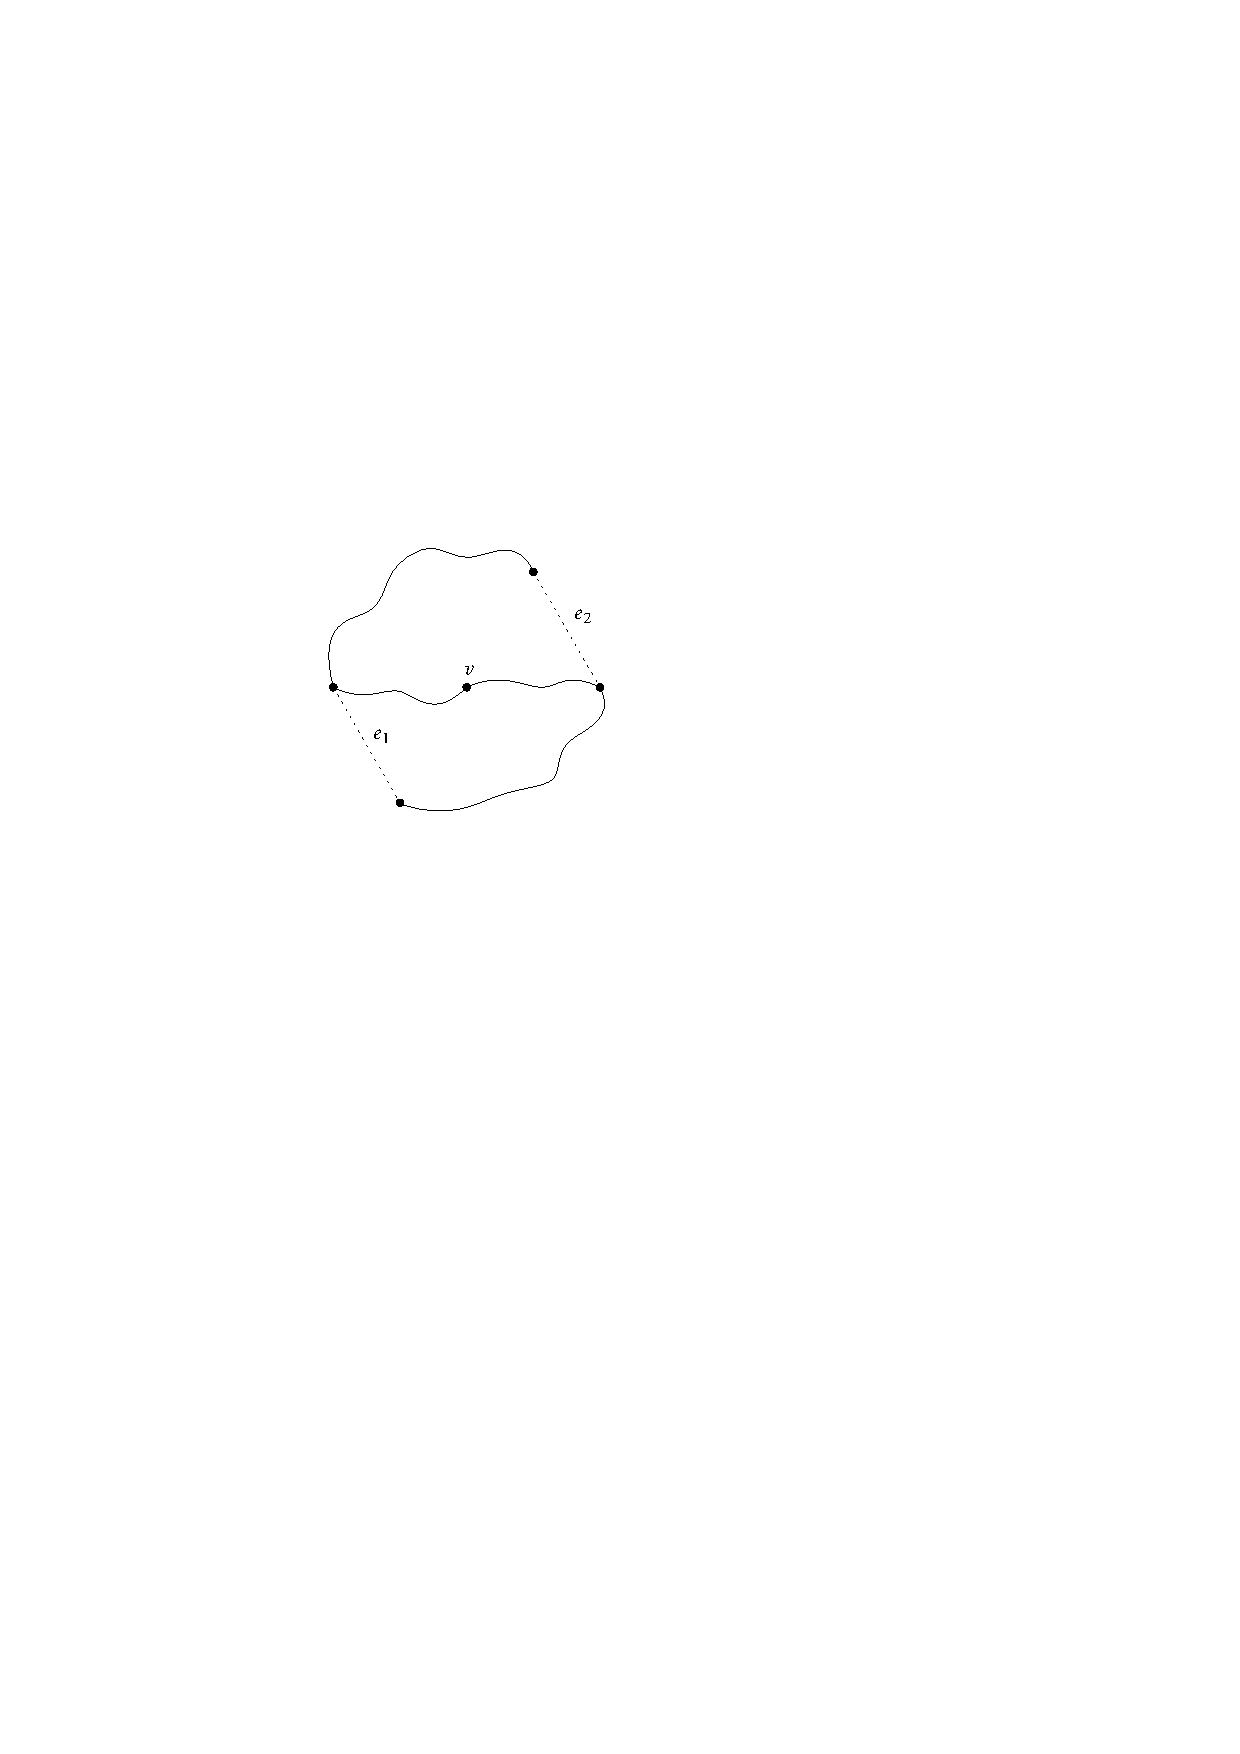
\includegraphics{cuckoo1}
      \caption{A cycle with a chord.}
    \end{subfigure}
    \quad\quad
    \begin{subfigure}[b]{0.6\textwidth}
      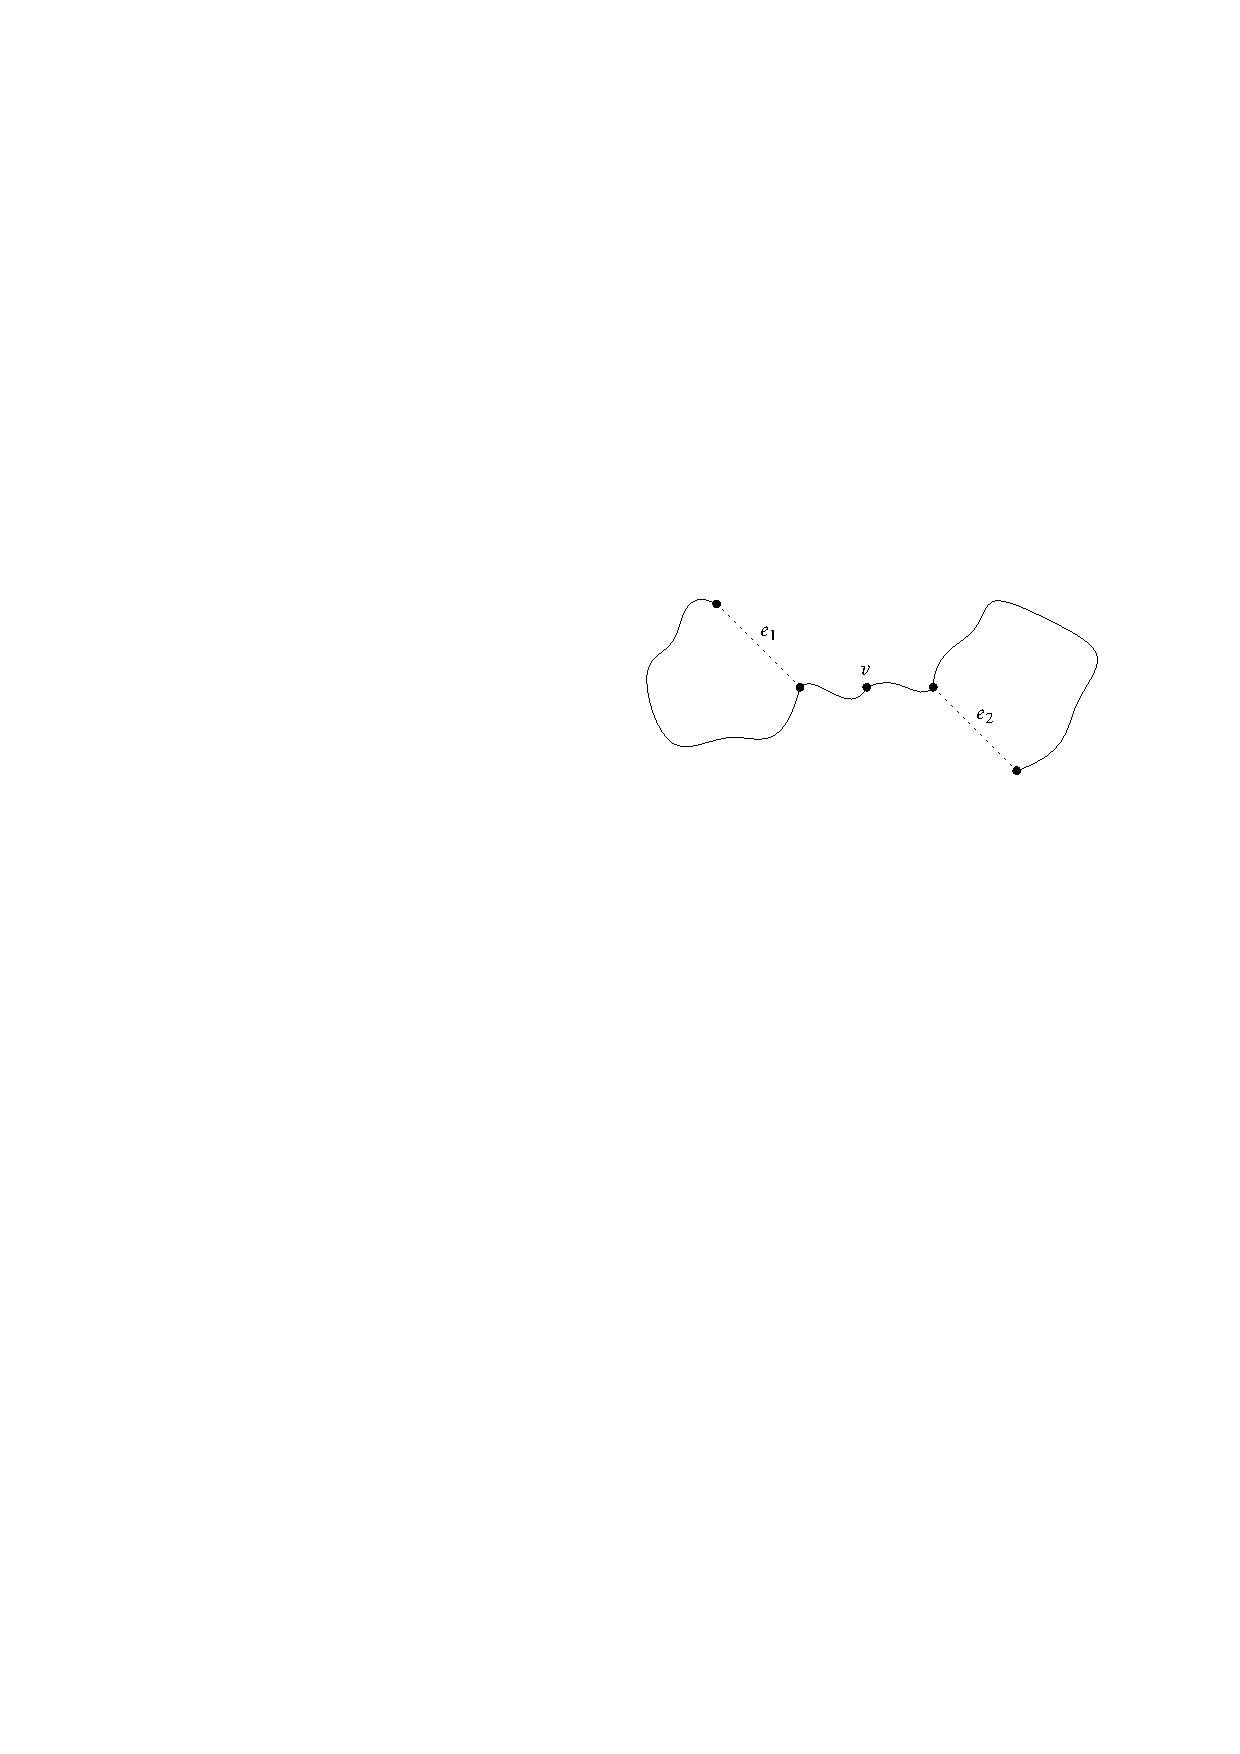
\includegraphics{cuckoo2}
      \caption{Two cycles connected by a path.}
    \end{subfigure}
    \caption{The potential minimal subgraphs of the cuckoo graph.}
    \figlabel{cuckoo-cycles}
  \end{figure}

  We encode $G$ by presenting Elias $\delta$-codes for the values of
  $t_1$ and $t_2$; then the edges of the above paths in order; then
  the vertices of the paths in order; and the edges $e_1$ and $e_2$;
  and finally the remaining $2n - 2(t + 1)$ endpoints of edges in the
  graph. Such a code has length
  \begin{align*}
    |C(G)| &\leq (t - 1)(\log n + \log m) + 2\log n + (2n - 2(t + 1))\log m + O(\log t) \\
           &= \log m^{2n} - 2\log m - t + O(\log t) \\
           &\leq \log m^{2n} - 2\log n + O(1) \enspace .
  \end{align*}
  We finish by applying the Uniform Encoding Lemma.
\end{proof}

From the union bound, we obtain the following:
\begin{cor}
  Cuckoo hashing succeeds upon insertion of $n$ elements with
  probability $1 - O(1/n)$.
\end{cor}

\subsection{2-Choice Hashing}

We showed in \secref{urns} that if $n$ balls are thrown independently
and uniformly at random into $n$ urns, then the maximum number of
balls in any urn is $O(\log n/\log \log n)$ with high probability. In
2-choice hashing, each ball is instead given a choice of two urns, and
the urn containing the fewer balls is preferred.

More specifically, we are given two hash functions
$h, g : X \to \{1, \ldots, m\}$. Each value of $h$ and $g$ points to
one of $m$ urns. The element $x \in X$ is added to the urn containing
the fewest elements between $h(x)$ and $g(x)$ during an insertion. The
worst case search time is at most the maximum number of hashing
collisions, or the maximum number of elements in any urn.

Perhaps surprisingly, the simple change of having two choices instead
of only one results in an exponential improvement over the strategy of
\secref{urns}. Indeed, 2-choice hashing was first studied by Azar
\emph{et al.}, who showed that the expected maximum size of an urn is
$\log \log n + O(1)$~\cite{azar:multiplechoice}. Our encoding argument
is based on V\"{o}cking's use of witness trees to analyze 2-choice
hashing~\cite{vocking:witness}.

Let $G = (V, E)$ be the random multigraph with $V = \{1, \ldots, m\}$,
where $m = cn$ for some constant $c \geq e$, and
$E = \{(h(x), g(x)) : x \in X\}$.

\begin{lem}
  The multigraph $G$ has an edge-simple path of length greater than
  $s + \log n + O(1)$ with probability at most $2^{-s}$.
\end{lem}
\begin{proof}
  We encode $G$ by presenting its set of edges. Since each endpoint of
  an edge of $G$ is independently chosen uniformly at random from $m$
  choices, then $G$ is chosen uniformly at random from a set of size
  $m^{2n}$.

  Suppose some vertex $v$ is the endpoint of an edge-simple path of
  length $t$. We encode this path by presenting the $t$ edges in
  order, including their orientation; then, the $t + 1$ vertices,
  starting from $v$; and finally, the remaining $2n - 2t$ endpoints of
  edges in the graph. Our code has length
  \begin{align*}
    |C(G)| &= t\log 2n + (t + 1)\log m + (2n - 2t)\log m \\
           &= 2n \log m + t \log 2n - t \log m + \log m + O(1) \\
           &= \log m^{2n} + t \log \frac{2n}{m} + \log m + O(1) \\
           &\leq \log m^{2n} - t \log (c/2) + \log n + O(1) \\
           &\leq \log m^{2n} - s \enspace ,
  \end{align*}
  as long as $t \log (c/2) \geq s + \log n + O(1)$, so apply the
  Uniform Encoding Lemma.
\end{proof}

\begin{lem}\lemlabel{two-choice-two-cycles}
  With probability $1 - O(1/n)$, $G$ has no subgraph with more edges
  than vertices.
\end{lem}
\begin{proof}
  Again, the proof is similar to that of \lemref{cuckoo-failure}, with
  an additional application of the union bound.
\end{proof}

\begin{lem}\lemlabel{two-choice-component-size}
  $G$ has a component of size at least $(2/\log(c/e))\log n + O(1)$
  with probability $O(1/n)$.
\end{lem}
\begin{proof}
  Suppose $G$ has a connected component $C$ with $t - 1$ edges and at
  most $t$ vertices. We encode the edge set of $G$ by providing the
  set of vertices in a spanning tree of $C$, and we choose to root
  this tree at the first vertex described in this set; then the shape
  of this tree; and the labels of the $t - 1$ edges encountered in an
  inorder traversal of this tree; and finally the remaining
  $2(n - t + 1)$ endpoints of edges. By Cayley's formula and since $G$
  is a multigraph, there are at most $t^{t - 2}$ rooted spanning trees
  of $G$. In total, our code has length
  \begin{align*}
    |C(G)| &= \log \binom{m}{t} + (t - 2) \log t + (t - 1) \log n + 2 (n - t + 1) \log m \\
           &\le 2n \log m + t\log m - t\log t + t\log e + (t-2)\log t + (t-1)\log n - 2(t-1)\log m & \text{(by \eqref{log-n-choose-k})} \\
           &\le 2n \log m - t\log c + t\log e - 2\log t + \log n + O(1) \\
           &\le \log m^{2n} - s \enspace ,
  \end{align*}
  as long as $t$ is such that
  \[t \log (c/e) + 2\log t \geq s + \log n + O(1) \enspace .\]
  In particular, if we choose $s = \log n$, applying \lemref{uel}
  tells us that $C$ has size at least $(2/\log (c/e))\log n + O(1)$
  with probability $O(1/n)$.
\end{proof}

Suppose that when $x$ is inserted, it is placed in a list with $t$
other elements. Then, we say that the age of $x$ is $a(x) = t$.
\begin{thm}
  The cost of any operation in 2-choice hashing is at most
  $\log \log n + O(1)$ with probability $1 - O(1/n)$.
\end{thm}
\begin{proof}
  Suppose that some element $x$ has $a(x) = t$. This leads to a binary
  \emph{witness tree} $T$ of height $t$ as follows.

  The root of $T$ is the element $x$. When $x$ was inserted into the
  hash table, it had to choose between the lists $h(x)$ and $g(x)$,
  both of which contained at least $t - 1$ elements; in particular,
  $h(x)$ has an element $x_h$ with $a(x_h) = t - 1$, and $g(x)$ has an
  element $x_g$ with $a(x_g) = t - 1$. The elements $x_h$ and $x_g$
  become left and right children of $x$ in $T$. The process continues
  recursively. If some element appears more than once on a level, we
  only recurse on its leftmost occurence.

  Note that each vertex of $T$ corresponds to the edge $(h(x), g(x))$
  of $G$. Moreover, the subgraph of $G$ induced by the edges
  $\{(h(x), g(x)) : x \in T\}$ is connected.

  Suppose that some node appears more than once on a level of
  $T$. From above, this means that some component of $G$ has a
  cycle. If this happens twice, then $G$ has a subgraph with more
  edges than vertices. By \lemref{two-choice-two-cycles}, this happens
  with probability $O(1/n)$.

  So with probability $1 - O(1/n)$, $T$ has at most one subtree
  removed, so $T$ has at least $2^t$ nodes. If we choose
  $t \ge \log \log n + d$, then $C$ has at least $2^d \log n$ nodes,
  which we know from \lemref{two-choice-component-size} happens with
  probability $O(1/n)$ for a sufficiently large choice of the constant
  $d$.
\end{proof}

\subsection{Robin-Hood Hashing}

Soon.


\subsection{Bipartite Expanders}

Consider a random bipartite multigraph $G=(A,B,E)$ where $|A|=|B|=n$
and the $3n$ edges in $E$ are obtained as follows:  Each vertex $u\in A$
chooses 3 random neighbours, $x(u)$, $y(u)$, and $z(u)$, in $B$, with
replacement.  All choices of edges are independent. For a set $A'\subseteq
A$, the \emph{neighbourhood} of $A'$, denoted $N(A')$, is the subset of
vertices in $B$ that are adjacent to at least one element of $A'$.

The following theorem shows that $G$ is an expander.  The proof of
this theorem usually involves a messy sum that contains binomial
coefficients and probabilities.  See, for example, Motwani and
Raghavan \cite[Theorem~5.3]{motwani.raghavan:randomized}, Pinsker
\cite[Lemma 1]{pinsker:on}, or Hoory, Linial, and Wigderson
\cite[Lemma~1.9]{hoory.linial.ea:expander}.

\begin{thm}
  There exists a constant $\alpha >0$ such that, with probability at
  least $O(n^{-1/2})$, $|N(A')| \ge 3|A'|/2$ for all $A'\subset A$
  with $|A'|\le \alpha n$.
\end{thm}

\begin{proof}
Without loss of generality, let $A=\{1,\ldots,n\}$.  We use an encoding argument on the bit string
\[
   R = x(1), y(1), z(1), x(2), y(2), z(2), \ldots, x(n), y(n), z(n) \enspace ,
\]
which is chosen uniformly from a set $X$ of size $n^{3n}$.

If some set $A'$, $|A'|=k\le \alpha n$, violates the conditions of the
lemma, then we encode $k$, $A'$, $N(A')$ and then the edges between
$A'$ and $N(A')$. Then we encode the rest of $R$, skipping the
$3k\log n$ bits devoted to elements in $A'$.  The key savings here
comes because $N(A')$ should take $3k\log n$ bits to encode, but can
actually be encoded in roughly $3k\log(3k/2)$ bits.

The total size of the first part of our encoding is, which includes $k$,
$A'$ and $N(A')$ is
\begin{align*}
    h & = 2\log k + \log\binom{n}{k} + \log\binom{n}{3k/2} + 3k\log (3k/2) \\
       & \le k\log n - k\log k + (3/2)k\log n - (3/2)k\log k + 3k\log k + k\log(3/2) \\
      & = (5/2)k\log n + (1/2)k\log k + k\log(3/2)  \enspace .
\end{align*}
The size of the second part of our encoding is $3n\log n - 3k\log n$.  The savings, $s=s(k)$, we obtain is therefore
\begin{align*}
     s(k) & = 3k\log n - (5/2)k\log n - (1/2)k\log k - k\log(3/2) \\
       & = (1/2)k(\log n - \log(2k/3)) \\
       & = (1/2)k(\log n - \log k - \log(3/2)) \\
       & = (1/2)k\log(2n/(3k)) \enspace .
\end{align*}
The function $s(k)$ is concave and is therefore minimized when $k$
is extremal, with the extremes being $k=1$ and $k=\alpha
n$. For $k=1$, we have
\[
    s(1)=(1/2)\log n - \log(2/3)
\]
and $2^{-s(1)} = O(n^{-1/2})$.  For $k=\alpha n$ we have
\[
   s(\alpha n) = (\alpha n/2)\log(2/(3\alpha))
\]
and $2^{-s(\alpha n)} = 2^{-\Omega(n)}$ for $\alpha < 2/3$.
\end{proof}

\subsection{Analysis of Insertion Sort}

Recall the insertion-sort algorithm for sorting a list, $A_1,\ldots,A_n$
of $n$ elements:

\noindent{$\textsc{InsertionSort}(A_1,\ldots,A_n)$}
\begin{algorithmic}[1]
  \FOR{$i\gets 2$ \TO $n$}
     \STATE{$j \gets i$}
     \WHILE{$j>1$ \AND $A_{j-1} > A_j$}
         \STATE{$A_j \leftrightarrow A_{j-1}$
            \COMMENT{ swap }}
         \STATE{$j\gets j-1$}
     \ENDWHILE
  \ENDFOR
\end{algorithmic}

A typical question asks the expected number of times Line~4 executes
if $A_1,\ldots,A_n$ is a uniformly random permutation of $n$ distinct
elements.  The answer $\binom{n}{2}/2$ is an easy application of
linearity of expectation: For every one of the $\binom{n}{2}$ pairs
$p,q\in\{1,\ldots,n\}$ with $p<q$, the values initially stored at
positions $A_p$ and $A_q$ will eventually be swapped if and only if $A_p >
A_q$, which happens with probability $1/2$ in a random permutation.

A more advanced question is to ask for a concentration result on the
number of executions of Line~4. This is a harder question to tackle;
because $>$ is transitive, the $\binom{n}{2}$ events being studied have
a lot of interdependence. In the following, we show how to obtain a
concentration result with an encoding argument.  The argument presented
here follows the same outline as Vitanyi's analysis of bubble sort
\cite{vitanyi:analysis}, though without all the trappings of Kolmogorov complexity.

\begin{thm}\thmlabel{insertion-sort}
  For a random permutation, $A_1,\ldots,A_n$ of $n$ distinct elements,
  the probability that Line~4 of \textsc{InsertionSort} executes fewer
  than $\alpha n^2 - n + 2$ times is at most $2^{n\log(\alpha e^2)+O(\log
  n)}$.  In particular, for a fixed $\alpha < 1/e^2$, this probability
  is $2^{-\Omega(n)}$.
\end{thm}

\begin{proof}
  Let $\pi$ be the permutation of $\{1,\ldots,n\}$ that defines the sorted
  order of $A_1,\ldots,A_n$, so that $A_{\pi_j}$ is the element that appears
  at position $j$ after sorting. Notice that $\pi$ is chosen uniformly at
  random among all $n!$ permutations of of $\{1,\ldots,n\}$.
  
  We encode the permutation $\pi$ by recording the execution of
  InsertionSort on this permutation. In particular, we record, for each
  $i\in\{2,\ldots,n\}$, the number of times, $m_i$, that Line~4 executes
  during the $i$th iteration of \textsc{InsertionSort}. With this information,
  one can run the following version of \textsc{InsertionSort} to recover $\pi$:
  
  \noindent{$\textsc{InsertionSortReconstruct}(m_2,\ldots,m_n)$}:
  \begin{algorithmic}[1]
    \STATE{$\pi \gets (1,\ldots,n)$}
    \FOR{$i\gets 2$ \TO $n$}
       \FOR{$j\gets i \textbf{ down to } i-m_i+1$}
           \STATE{$\pi_j \leftrightarrow \pi_{j-1}$
              \COMMENT{ swap }}
       \ENDFOR
    \ENDFOR
  \end{algorithmic}
   
  To make this work, we have to be slightly clever with this
  encoding. Rather than encode $m_2,m_3,\ldots,m_n$ directly, we first
  encode $m=\sum_{i=2}^{n} m_i$ using $\lceil 2\log n\rceil$ bits (since $m < n^2$). Given $m$, what
  remains is to describe the partition of $m$ into $n-1$ non-negative
  integers $m_2,\ldots,m_n$; there are $\binom{m+n-2}{n-2}$ such
  partitions.\footnote{To see this, draw $m+n-2$ white dots on a line,
  then choose $n-2$ dots to colour black. This splits the remaining $m$ white dots
  up into $n-1$ groups, which determine the values of $m_2,\ldots,m_n$.}
  
  Therefore, the values of $m_2,\ldots,m_n$ can be encoded using
  \[
      b = \lceil 2\log n\rceil + \log\binom{m+n-2}{n-2}
  \]
  bits and this is sufficient to recover the permutation that defines
  $A_1,\ldots,A_n$.  By applying \eqref{log-n-choose-k} to $b$, we obtain
  \begin{align*}
    b & \le (n-2)\log(m+n-2) - (n-2)\log(n-2)  + (n-2)\log e + O(\log n) \\
      & \le n\log(m+n-2) - n\log n   + n\log e + O(\log n) \\
      & \le n\log(\alpha n^2) - n\log n  + n\log e + O(\log n) \\
      & = 2n\log n + n\log\alpha - n\log n  + n\log e + O(\log n) \\
      & = n\log n + n\log\alpha + n\log e + O(\log n) \\
      & = \log n! + n\log\alpha + 2n\log e + O(\log n) \\
      & = \log n! + n(\log \alpha e^2) + O(\log n)  \qedhere
  \end{align*}
\end{proof}

\begin{rem}
  Although it doesn't require any advanced probability,
  \thmref{insertion-sort} is not sharp; it only gives a non-trivial
  probability when $\alpha < 1/e^2$.  To obtain a sharp bound, one can
  use the fact that $m_2,\ldots,m_n$ are independent and $m_i$ is uniform
  over $\{0,\ldots,i-1\}$ and then use the method of bounded differences
  \cite{mcdiarmid:on} to show that $m$ is concentrated in an interval
  of size $O(n^{3/2})$.
\end{rem}

\subsection{Permutation Statistics}

We consider the use of encoding arguments to study statistics of
equiprobable permutations of $\{1, 2, \ldots, n\}$.

\subsubsection{Records}

Figure out where to move Shannon-Fano code stuff here.  

\subsubsection{The Height of Random Binary Search Tree}

\subsubsection{Hoare's Find Algorithm}


\section{The Non-Uniform Encoding Lemma and Shannon-Fano Codes}
\seclabel{nuel}

Thus far, we have been lucky to study applications that could always
be modelled as choosing some element $x$ uniformly at random from a
set $X$. To encompass even more applications, it is helpful to have
an Encoding Lemma that deals with non-uniform distributions over $X$.
The following generalization of the Uniform Encoding Lemma fills this
need:

\begin{lem}[Non-Uniform Encoding Lemma]\lemlabel{nuel}  
  Let $C\from X\to\{0,1\}^*$ be a prefix code and let $x\in X$ be
  drawn randomly where $p_x$ denotes the probability of drawing $x$.
  Then $\Pr\{ |C(x)| \le \log(1/p_x)-s\} \le 2^{-s}$.
\end{lem}

\begin{proof}
  We use Chernoff's trick, Markov's Inequality, and Kraft's Inequality,
  as follows: 
  \begin{align*}
     \Pr\{ |C(x)| \le\log(1/p_x)-s \} 
      & = \Pr\{|C(x)| -\log(1/p_x) \le -s \} \\
      & = \Pr\{\log(1/p_x)-|C(x)| \ge s \} \\
      & = \Pr\left\{2^{\log(1/p_x)-|C(x)|} \ge 2^s \right\} & \text{(Chernoff's trick)} \\
      & \le \frac{\E\left[2^{\log(1/p_x)-|C(x)|}\right]}{2^s} & \text{(Markov's Inequality)} \\
      & = \frac{\sum_{x\in X}p_x\cdot 2^{\log(1/p_x)-|C(x)|}}{2^s} \\
      & = \frac{\sum_{x\in X}2^{-|C(x)|}}{2^s} \\
      & \le \frac{1}{2^s} & \text{(Kraft's Inequality).}  & \qedhere
  \end{align*}
\end{proof}

Notice that the Non-Uniform Encoding Lemma is a strict generalization
of the Uniform Encoding Lemma; take $p_x=1/|X|$ for all $x\in X$
and we obtain the Uniform Encoding Lemma.

The \emph{Shannon-Fano code} \cite{fano:transmission,shannon:mathematical}
for a finite set $X$ is prefix-free code that is constructed by a top-down
algorithm from a probability distribution over the elements of $X$. An
important property of the Shannon-Fano code is that it is \emph{locally
optimal}: If $C\from X\to\{0,1\}^*$ is a Shannon-Fano code, then for every $x\in X$,
\[
    |C(x)| \le \left\lceil\log(1/p_x)\right\rceil \enspace 
\]
where, as before, $p_x$ denotes the probability of $x$.

When designing efficient encoding schemes it helps, at least
informally, to think of $\log(1/p)$ as the cost of encoding a 1 bit and
$\log(1/(1-p))$ as the cost of encoding a 0 bit.  For example, $p=1/n$

We will find it particularly useful to apply Shannon-Fano codes to
$\mathrm{Bernoulli}(p)$ strings consisting of indepenent random bits that
are each set to 1 with probability $p$ and 0 with probability $1-p$.
A particular binary string $x=x_1,\ldots,x_n$, occurs as
a $\mathrm{Bernoulli}(p)$ string with
probability exactly
\[
   p_x= p^{r_1}(1-p)^{r_0} \enspace ,
\]
where $r_1$ and $r_0$ are the numbers of 1 and 0 bits in $x$, respectively. In this case, the Shannon-Fano code for $x$ has length at most
\[
    |C(x)|\le \left\lceil r_1\log (1/p) + r_0\log(1/(1-p)) \right\rceil \enspace .
\]


\section{Applications of the Non-Uniform Encoding Lemma}
\seclabel{applications-ii}

\subsection{Chernoff's Bounds}
\seclabel{chernoff}

The following theorem is the so-called \emph{additive version} of the
Chernoff bound on the tail of a binomial random variable:

\begin{thm}\thmlabel{chernoff}
  If $B$ is a $\mathrm{binomial}(n,p)$ random variable, then $\Pr\{B\ge
  (p+\epsilon)n\} \le 2^{-nD(p+\epsilon||p)}$, where 
  \[ 
    D(\hat p||p)=\hat p\log(\hat p/p) + (1-\hat p)\log((1-\hat p)/(1-p)) 
  \] is
  the Kullbach-Liebler divergence between Bernoulli random variables
  with probabilities $\hat p$ and $p$.
\end{thm}

\begin{proof}
By definition, $B=\sum_{i=1}^nx_i$, where $x_1,\ldots,x_n$ are independent $\mathrm{Bernoulli}(p)$ random variables.   We will use an encoding argument on the bitstring $x=x_1,\ldots,x_n$.

We can encode $x$ by using a Shannon-Fano code for the probability
$p+\epsilon$.  If $B=\hat pn$, then this takes
\[
   b = n(\hat p\log(1/(p+\epsilon))+ (1-\hat p)\log(1/(1-p-\epsilon)))
\]
bits.

On the other hand,
\[
    p_x = p^{\hat pn}(1-p)^{(1-\hat p)n} \enspace ,
\]
and
\[
    \log (1/p_x) = n(\hat p\log(1/p)+ (1-\hat p)\log(1/(1-p)) \enspace .
\]
For $\hat p\ge p+\epsilon$, the savings from this code is
\begin{align*}
  \log(1/p_x) - b
    & =  n(\hat p\log((p+\epsilon)/p) + (1-\hat p)\log((1-p-\epsilon)/(1-p))) \\
    & \ge  n((p+\epsilon)\log((p+\epsilon)/p) + (1-p-\epsilon)\log((1-p-\epsilon)/(1-p)))\\
    & =  nD(p+\epsilon||p)
\end{align*}
bits.  Therefore, the probability that $B\ge (p+\epsilon)n$ is at most $2^{-nD(p+\epsilon||p)}$.
\end{proof}

It is also possible to derive the multiplicative form of the Chernoff
bound this way. This is left an exercise to the reader.

\subsection{Percolation on the Torus}

The following is a version of Peierls' argument that proves that
percolation occurs on the torus if the edge survival rate is greater
than $2/3$:

\begin{thm}
  Let $G$ be the $\sqrt n\times\sqrt n$ torus and let $G'$ be the graph
  obtained by sampling each edge of $G$ independently with probability
  $p<1/3$.  Then the probability that $G'$ contains a simple cycle of
  length at least $t=(s+\log n+O(1))/\log(1/(3p))$ is at most $2^{-s}$.
\end{thm}

\begin{proof}
  Let $x$ be the bitstring of length $r=2n$ that encodes the existence
  of the edges in $G'$.  Suppose such a cycle, $C$, exists in $G'$
  and its length is $t'$.  Then we can encode $G'$ by specifying a
  single vertex, $u$, on $C$; the sequence of $t'$ steps (directions)
  that the cycle moves along from there; and then the rest of $G$ using
  a variable length code with parameter $p$.

  When specifying the cycle, there are four possibilities for the first
  step, but only three possibilities for each the subsequent step. Therefore,
  all the steps in the cycle can be specified using $\lceil 2+(t'-1)\log
  3\rceil$ bits.

  The total lenght of the codeword is then
  \[
      b = \log n + t'\log 3 + (r_1-t')\log(1/p) + r_0\log(1/(1-p)) + O(1) 
  \]
  bits, where $r_1$ is the number of edges in $G'$ and $r_0=r-r_1$
  is the number of missing edges in $G'$.  But then,
  \[
     p_x = p^{r_1}(1-p)^{r_0}
  \]
  so 
  \[
     \log(1/p_x) = r_1\log(1/p) + r_0\log(1/(1-p)) \enspace .
  \]
  Therefore, $\log(1/p_x)-b = t'(\log(1/p)-\log 3) - \log n - O(1)\ge
  s$, for $t'\ge t$.  Applying the Non-Uniform Encoding Lemma completes
  the proof.
\end{proof}

Since the torus is self-dual, this implies that if we keep each edge of the torus with probability greater than $2/3$ then, with high probability, there is only one component whose size is $\omega(\log^2 n)$.  This is because, having more than one such component would imply the existence of a dual cycle of missing edges whose length is $\omega(\log n)$.  The preceding theorem shows that, with high probability, no such dual cycle exists.


\subsection{Triangles in $G_{n,p}$}

The expected number of triangles (cycles of length 3) in $G_{n,p}$
is easily seen to be $p^3\binom{n}{3}$.  For $p=(6k)^{1/3}/n$, this
expectation is $k-O(1/n)$.  Unfortunately, even when $k$ is a large
constant, it still takes some work to show that there is a constant
probability that $G_{n,p}$ contains at least one triangle. Indeed, this
typically requires the use of the second moment method, which involves
computing the variance of the number of triangles in $G_{n,p}$.

Here we show how this can be accomplished with an encoding argument.

\begin{thm}
  For $p=c/n$, $G_{n,p}$ contains at least one triangle with probability
  at least $1-2^{-\Omega(c^3)}$.
\end{thm}

\begin{proof}
   Without loss of generality assume that $G$'s vertex set is
   $V=\{1,\ldots,n\}$.  In this argument, we will produce an encoding
   of $G$'s adjacency matrix, $x$.

   Refer to \figref{triangles}.  If $G$ contains no triangles, then we
   look at the number of 1's in the $n/2\times n/2$ submatrix
   determined by rows $1,\ldots,n/2$ and columns $n/2+1,\ldots,n$.
   There are two cases to consider (which result in codewords
   beginning with 10 or 11, respectively):

   \begin{figure}
     \centering{\includegraphics{triangles}}
     \caption{The random graph $G_{n,c/n}$ contains triangles when $c$ is
       large enough.  The highlighted 0 bits in the last five rows can
       be deduced from pairs of 1 bits in the first 5 rows.}
     \figlabel{triangles} 
   \end{figure}

   \begin{enumerate}\setcounter{enumi}{-1}
     \item The number of 1's in the submatrix is less than $cn/8$.
      In this case, the number of 1's in this submatrix is much less than
      the expected number, $cn/4$.  Here one can apply the same argument
      used to prove Chernoff's Bounds (\thmref{chernoff}) or simply
      apply Chernoff's bounds. We leave this as an exercise to the reader.

     \item The number of 1's in the submatrix is greater than $cn/8$.
      Notice that, for $i<j<k$ if $M_{i,j}=1$ and $M_{i,k}=1$, then the
      fact that there are no triangles implies tha $M_{j,k}=0$.

      Let $m_i$ be the number of 1's in the $i$th row of the submatrix.
      By specifying rows $1,\ldots,n/2$, we eliminate the need to specify
      \[
          m = \sum_{i=1}^{n/2}\binom{m_i}{2} \ge (n/2)\binom{c/4}{2} = \Omega(c^2n) \enspace ,
      \]
      zeros in rows $n/2+1,\ldots,n$.
      Using a Shannon-Fano code to specify the first $n/2$ rows and the bits of the remaining rows that can not be deduced from the first $n/2$ rows, we obtain a codeword of length 
      \[
          b = r_1\log(1/p) + (r_0-m)\log(1/(1-p))  + O(1)
      \]
      which results in a savings of
      \[
          s = \log(1/p_x) - b = m\log(1/(1-p)) -O(1) \ge \Omega(c^2n)\log(1/(1-p)) - O(1) = \Omega(c^3) \enspace .
      \]
   \end{enumerate}
\end{proof}


\subsection{The Components of $G_{n,p}$}

[The following result is really boring. It's easier to prove just using linearity of expectation and Markov's Inequality.]

\begin{thm}
  For $p=\alpha/n$, the probability that $G_{n,p}$ contains a component of size at least $t$ is at most $blah$.
\end{thm}

\begin{proof}
  We use an encoding argument on the bits of the adjacency matrix, $x$,
  of $G$.

  If $G$ does contain a component of size $t$ or greater, then we
  find, within this component, a tree, $T$, of size exactly $t$.  The
  codeword then consists of a list of the vertices in $T$ as they are
  encountered during an preorder traversal, a description of the shape
  of $T$, and then finally, a Shannon-Fano code that gives the
  $\binom{n}{2}-t+1$ bits of the adjacency matrix corresponding to the
  edges not in $T$.

  The shape of $T$ can be described using $2n$ bits by tracing the
  execution of the traversal of $T$, using a 1 to indicate that the
  traversal takes a step deeper into the tree and a 0 to indicate that
  the traversal moves up in the tree.

  In total, this results in a codeword of length
  \[   
    b \le 2 + t\log n + 2t + (r_1-t+1)\log(1/p) + r_0\log(1/(1-p))  \enspace . 
  \]
  On the other hand
  \[   
     \log (1/p_x) = r_1\log(1/p) + r_0\log(1/(1-p)) \enspace ,
  \]
  so
  \begin{align*}
     s & = \log(1/p_x) - b \\
       & =  (t-1)\log(1/p) - t\log n - 2t - 2 \\
       & = t(\log(1/p)-\log n - 2) - \log n - 2 \\
       & = t\log(1/(4\alpha)) - \log n - 2 \\
  \end{align*}
\end{proof}

[This is also really boring\ldots]

\begin{lem}
  The probability that $G_{n,p}$ has a partition of $(U,W)$ of its vertex
  set such that $|U|=k$ and there is no edge with one endpoint in $U$
  and one endpoint in $W$ is at most $2n^k\cdot (1-p)^{k(n-k)}$.
\end{lem}

\begin{proof}
  We encode the adjacency matrix, $x$, of $G_{n,p}$ as follows.
  If $G_{n,p}$ does not contain such a partition, then the encoding is
  zero bit followed by the obvious encoding.

  Otherwise, the encoding is a one bit, followed by the list of $k$
  vertices, followed by the remaining $\binom{n}{2}-k(n-k)$ bits of the
  adjacency matrix that are not implied by the information already given.
  These latter bits are encoded using a Shannon--Fano code that is
  optimized for $p$.

  If $G$ has $r_1$ edges and $r_0=\binom{n}{2}-r_1$ non-edges, then the codeword has length
  \begin{align*}
      b & = 1 + k\log n + r_1\log(1/p) + (r_0-k(n-k))\log(1/(1-p)) \enspace .
  \end{align*}
  On the other hand,
  \[
      \log p_x = r_1\log(1/p) + r_0\log(1/(1-p)) \enspace ,
  \]
  so the savings obtained by this encoding is 
  \[
      s = \log p_x - b = k(n-k)\log(1/(1-p)) - k\log n - 1 \enspace ,
  \]
  and the result follows from the Non-Uniform Encoding Lemma.
\end{proof}




\subsection{}


\section{Weight Functions}
\seclabel{weights}

\section{Summary and Conclusions}
\seclabel{summary}


\section*{Acknowledgement}

This research was initiated in response to an invitation to give
a talk at the Ninth Annual Probability, Combinatorics and Geometry
Workshop, held April 4--11 at McGill University's Bellairs Institute.
Many ideas that appear in the current paper were developed during the
workshop. The author is grateful to the other workshop participants for
providing a stimulating working environment.  In particular, Xing~Shi~Cai
pointed out the application to runs in binary strings (\thmref{runs-i})
and G\'abor~Lugosi stated and proved the Non-Uniform Encoding Lemma
(\lemref{nuel}) in response to the author's half-formed ideas about a
non-uniform version of \lemref{uel}.

\bibliographystyle{plain}
\bibliography{encoding}

\end{document}
